% Chapter 3

\chapter{Methodology}

\label{Chapter3} % For referencing the chapter elsewhere, use \ref{Chapter3} 

\section{Development Approach}

While starting the project, we had two methods or idealogies to go by
either following a waterfall model or an agile model. The waterfall model
is a sequential design process, used in software development processes,
in which progress is seen as flowing steadily downwards (like a waterfall)
while the agile model is a practice that promotes continuous iteration of
development and testing throughout the software development lifecycle of the
project. Both of these models have their own advantages and disadvantages.\par\medskip

After careful consideration, we decided to go with a Hybrid model which is a
combination of both waterfall and agile model. Initially, we followed a Waterfall approach
for planning and designing phases of the project. After the planning and designing phase,
we tranisitioned to an agile model for the development phase of the project. This approach
helped us to have a clear idea of what we were going to do and how we were going to do it by
implementing the features in sprints, continuosly monitoring the resultings, analyzing data, and making
adjustments.

\section{Iterations and Sprints}
Our application development journey was organized into distinct sprints, each focusing on pivotal components vital to our renting platform's functionality and user experience.\par\medskip
\clearpage

\textbf{Sprint 1: Onboarding Experience}
In this sprint, our emphasis was on crafting a seamless onboarding flow. We concentrated on creating an intuitive and user-friendly registration process, ensuring users effortlessly navigate through initial setup, profile creation, and account authentication.\medskip

\textbf{Sprint 2: Dynamic Dashboard Design}
Our team dedicated this sprint to developing a dynamic and informative dashboard. Here, the focus was on designing an interface that offers users a comprehensive overview of their rented properties, team collaborations, and reminders, fostering a centralized hub for efficient property management.\medskip

\textbf{Sprint 3: Room Rental \& Roommate Finder Logic}
In this sprint, the spotlight was on formulating and implementing robust logic for room rental and roommate finder functionalities. We concentrated on refining algorithms that power property searches, match roommates based on preferences, and streamline the rental process for individual users and collaborative teams.\medskip

\textbf{Sprint 4: AI-Driven Price Prediction Model}
A critical phase, this sprint was dedicated to integrating an AI-driven price prediction model. We meticulously crafted and integrated machine learning algorithms to provide accurate rental price estimations, enhancing transparency and aiding users in making informed decisions.\medskip

\textbf{Sprint 5: Team Invitation Management}
Here, our focus shifted towards creating and implementing the logic necessary to create and manage team invitations effectively. We engineered a system that allows users to form collaborative teams seamlessly, enabling efficient property searches and shared responsibilities among team members.\medskip

\textbf{Sprint 6: Robust Chat System}
The final sprint concentrated on the development of a robust chat system. We engineered a communication platform that fosters seamless interaction between users, facilitating easy communication within collaborative teams, aiding in decision-making, and enhancing overall user engagement.\par\bigskip

These delineated sprints encapsulate the strategic breakdown of our development process, allowing us to iteratively build, test, and refine specific components of our renting application, culminating in a comprehensive and user-centric platform.

\section{Tools and Technologies}

\subsection{Programming Languages and Frameworks}

\textbf{Next.js Framework with TypeScript:}
Our renting application was built upon the Next.js framework, utilizing TypeScript for enhanced type safety and code clarity. Next.js, combined with TypeScript, empowered us to develop a robust, scalable, and statically typed application, ensuring improved code quality and developer productivity.

\medskip\noindent
\textbf{Shadcn UI Components:}
Shadcn UI components played a pivotal role in expediting the frontend development process. These pre-designed components, coupled with TypeScript support, facilitated rapid UI development, ensuring consistency and aesthetic appeal across the application.

\medskip\noindent
\textbf{React-Hook-Forms with Zod Validators:}
For efficient form management and data validation, we integrated React-Hook-Forms with Zod validators. This amalgamation, leveraging TypeScript's typing capabilities, allowed for seamless form handling, validation, and data integrity checks.

\subsection{Development Tools}
\textbf{VSCode Editor:}
Visual Studio Code (VSCode) remained our IDE of choice, offering a robust development environment with TypeScript support. Its extensive feature set, including debugging tools and TypeScript linting, facilitated efficient coding practices and collaboration among team members.

\medskip\noindent
\textbf{Git/GitHub Version Control:}
Git in conjunction with GitHub served as our version control system, allowing collaborative development and code management. TypeScript's typing features integrated seamlessly with Git, aiding in version tracking and ensuring code consistency.

\medskip\noindent
\textbf{Vercel for Deployment:}
Vercel's deployment platform, compatible with TypeScript and Next.js, streamlined our deployment process. This powerful platform facilitated quick and reliable deployment, ensuring that updates were efficiently pushed to production with TypeScript support.

\medskip\noindent
\textbf{Docker}
Docker was used to run supabase locally for running supabase-cli scripts to update database migration files.

\subsection{Database Management:}
\textbf{Supabase:}
Postgres-Based DB with Buckets for Data and Image Storage;
Supabase, integrated with TypeScript for seamless data handling, functioned as our primary database solution. The PostgreSQL-based database, coupled with TypeScript's typing features, provided a secure and scalable infrastructure for storing application data and images through Supabase buckets.

\section{Development Process}

This section will summarize the development process, including how we approached the problems technically.

\subsection{Setup}

The project was initialized using create-next-app with the supabase template.\medskip
\begin{lstlisting}[language=bash]
    npx create-next-app -e with-supabase
\end{lstlisting}

\subsubsection{Cookie-based Auth}
We are using Cookie-based Auth in our web application. The Next.js Auth Helpers package configures Supabase Auth to store the user's session in a cookie, rather than localStorage. This makes it available across the client and server of the App Router - Client Components, Server Components, Server Actions, Route Handlers and Middleware. The session is automatically sent along with any requests to Supabase.\smallskip

\begin{lstlisting}[language=bash, caption={Installing Auth Helpers}]
npm install @supabase/auth-helpers-nextjs @supabase/supabase-js
\end{lstlisting}
\noindent
We are then declaring environment variables in .env.local file with following environment variables:
\begin{lstlisting}[caption={.env.local}]
    NEXT_PUBLIC_SUPABASE_URL=your-supabase-url
    NEXT_PUBLIC_SUPABASE_ANON_KEY=your-supabase-anon-key
\end{lstlisting}

The Next.js Auth Helpers are configured to use the server-side auth flow to sign in users
into the application. For this we had to setup a Code Exchange route, to exchange an auth
code for the user's session, which is set as a cookie for future requests made to Supabase.

We created a callback route handler that performs this exchange at app/api/auth/callback/route.js:

\begin{lstlisting}[language=javascript, caption={Callback Route Handler}]
import { createRouteHandlerClient } from '@supabase/auth-helpers-nextjs'
import { cookies } from 'next/headers'
import { NextResponse } from 'next/server'

export async function GET(request) {
  const requestUrl = new URL(request.url)
  const code = requestUrl.searchParams.get('code')

  if (code) {
    const cookieStore = cookies()
    const supabase = createRouteHandlerClient({ cookies: () => cookieStore })
    await supabase.auth.exchangeCodeForSession(code)
  }


  // URL to redirect to after sign in process completes
  return NextResponse.redirect(requestUrl.origin)
}
\end{lstlisting}
\clearpage
Part of inviting users to our application was having a attractive UI. We achieved this
through discussing over design language and then finalising over shadcn's collection for our UI components. Shadcn-ui contains re-usable components built using Radix UI and Tailwind CSS.

\subsubsection{Dark Mode Support}
We are using next-themes package to support dark mode in our application. This package provides a useTheme hook that allows us to access the current theme and toggleTheme function to toggle between light and dark mode. We are using this hook to toggle between light and dark mode in our application.

\begin{lstlisting}[language=bash, caption={Installing next-themes}]
    npm install next-themes    
\end{lstlisting}

\noindent Creating a theme provider\par\medskip\noindent
components/theme-provider.tsx

\begin{lstlisting}[language=javascript, caption={Theme Provider}]
"use client"

import * as React from "react"
import { ThemeProvider as NextThemesProvider } from "next-themes"
import { type ThemeProviderProps } from "next-themes/dist/types"
    
export function ThemeProvider({ children, ...props }: ThemeProviderProps) {
    return <NextThemesProvider {...props}>{children}</NextThemesProvider>
}
    
\end{lstlisting}

The created theme-provider is added to the root layout and linked with tailwind-css config file to achieve the proper result.

\clearpage
\subsection{Database Structure and Functionality}

\begin{figure}[h]
    \centering
    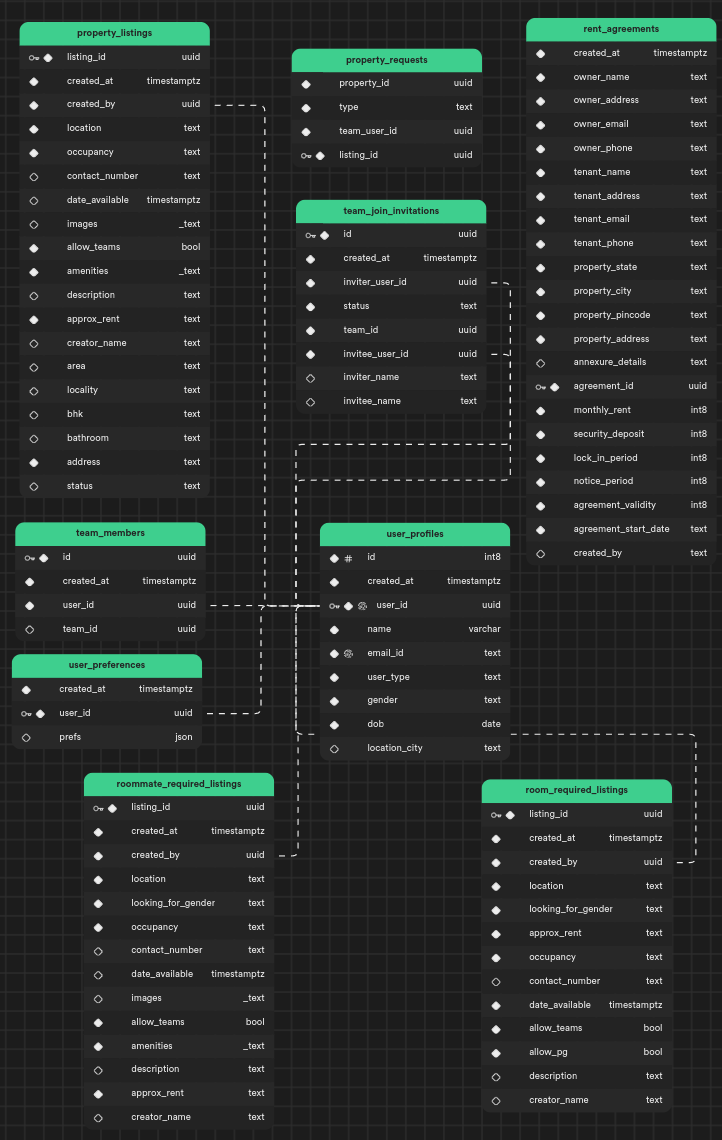
\includegraphics[width=0.7\textwidth]{Images/schema_visualizer.png}
    \caption{Funding trend analysis}
\end{figure}
This image describes the database structure of our application. We have used supabase's database and storage buckets to store our data. We have used supabase's auth to authenticate users and supabase's storage buckets to store images and other files.
\clearpage

\subsubsection{Why Supabase and PostgreSQL?}

\noindent\textbf{Utilizing Row-Level Security (RLS) Policies}
\par\smallskip\noindent One of the key features that drew us to Supabase is its implementation of Row-Level Security (RLS) policies. RLS policies enable fine-grained control over data access within the database by restricting users' access to specific rows based on defined security policies.

In our room renting application, RLS policies play a pivotal role in ensuring data security and privacy. They allow us to enforce access control mechanisms at the row level, granting users access only to the data relevant to their interactions and permissions. For instance, RLS policies dictate that users can view and interact with property listings, roommate preferences, or matchmaking data only within the scope of their authorized permissions, enhancing data confidentiality and integrity.

\par\medskip
\noindent\textbf{Triggers in PostgreSQL}
\par\smallskip\noindent PostgreSQL's robust support for triggers serves as a pivotal element in automating various processes within the database. Triggers enable the execution of predefined actions in response to specific database events, ensuring streamlined and automated workflows.

In our application, triggers play a pivotal role in orchestrating interactions between users and property listings, facilitating personalized recommendations, and triggering roommate matchmaking processes. For instance, when a user expresses interest in a property or updates their preferences, triggers activate functions that analyze compatibility, recommend suitable listings, or initiate matchmaking processes.

\par\medskip
\noindent\textbf{PL/pgSQL Functions for Automation}
\par\smallskip\noindent The integration of PL/pgSQL functions within PostgreSQL further amplifies the automation capabilities of our database. PL/pgSQL, a procedural language extension for PostgreSQL, allows the creation of custom functions to automate complex database operations.

These functions empower our system to automate tasks such as automatically moving members to correct teams after they accept or decline an invite request.

\clearpage
\subsubsection{Team Invitation Management}

Users can browser other users who have signed up for teams and filter them based on the their preferences, the preferences were already
stored during onboarding and are used to calculate a score for each user. The score is calculated by comparing the user's preferences with the
preferences of the user who is searching for a roommate.\par

We are mainly taking advantage of two tables in our schema for this purpose, team\_members and team\_join\_invitations. The team\_members table
contains mapping of users to teams and the team\_join\_invitations table contains list of all the invitations sent to users to join a team, with a column
having the status of the invite as "waiting", "accepted" or "rejected".\par
\medskip
\noindent We have a postgres trigger in place watching over the value of status and it is triggered when the value of status changes from "waiting" to "accepted".

\begin{lstlisting}[language=sql]
CREATE TRIGGER "on_team_invitation_accepted_trigger"
AFTER
UPDATE ON "public"."team_join_invitations" FOR EACH ROW
    WHEN (
    (
        ("old"."status" <> "new"."status")
        AND (
        "new"."status" = 'accepted'::"text"
        )
    )
) EXECUTE FUNCTION "public"."handle_add_team_member_after_invitation_accepted"();
\end{lstlisting}

\noindent The trigger calls a function handle\_add\_team\_member\_after\_invitation\_accepted which adds the user to the team and updates the values in team\_members table.
\begin{lstlisting}[language=sql]
create function "public"."handle_add_team_member_after_invitation_accepted" () returns "trigger" language "plpgsql" security definer as $$BEGIN
UPDATE team_members
SET team_id = NEW.team_id
WHERE user_id = NEW.invitee_user_id;
    
IF NOT FOUND THEN
INSERT INTO team_members(user_id, team_id)
VALUES (
    NEW.invitee_user_id,
    NEW.team_id
    );
END IF;
RETURN NEW;
END;
$$;
\end{lstlisting}

\noindent The changes are then reflected in the application and the user is added to the team.

\subsection{Rent Agreement Generation}

The implementation of a multi-step form using the useMultiStepForm React hook stands as a cornerstone in our room renting application, specifically facilitating the seamless input of data required for generating rent agreements in PDF format. This client-side process employs the react-pdf package for PDF generation and utilizes file-saver to enable users to download the finalized agreement.\par\medskip

\noindent
\textbf{Functionality of the Mutli-Step Form}\par\medskip\noindent
The useMultiStepForm hook was custom-built to guide users through a structured sequence of input fields necessary for creating a comprehensive rent agreement. Each step of the form collects specific information, such as:

\begin{itemize}
    \item Agreement details
    \item Tenant details
    \item Owner details
    \item Property details
    \item Additional details
\end{itemize}
\noindent
The structured nature of the multi-step form ensures that users provide all necessary information required to generate a legally binding rent agreement.

\medskip
\noindent
\textbf{Rent Agreement Download}\par\medskip\noindent
Upon completion of the multi-step form, the entered data is compiled and processed client-side using the react-pdf package. This package dynamically generates a PDF document based on the collected input, encapsulating the terms and clauses specified in the rent agreement.\par\medskip

Subsequently, the file-saver library is utilized to enable users to download the generated rent agreement PDF directly from the client-side interface, providing a convenient and immediate access method for users.

\medskip
\noindent
\textbf{Status of Digital Agreements in Indian Law}\par\medskip\noindent
In India, the status of digital agreements is governed by the Information Technology Act, 2000, and the Indian Contract Act, 1872. These legal frameworks recognize electronic documents and digital signatures as valid and enforceable, provided they comply with specific requirements, including:

\begin{itemize}
    \item Authentication of electronic records
    \item Ensuring the integrity of the information
    \item Obtaining consent from involved parties
\end{itemize}
Digital agreements, including electronically signed rent agreements, hold legal validity if they adhere to these stipulations outlined in Indian law.

\subsection{AI-Driven Price Prediction Model}

\subsubsection{Context}
Housing in India varies from palaces of erstwhile maharajas to modern apartment buildings in big cities to tiny huts in far-flung villages. There has been tremendous growth in India's housing sector as incomes have risen. The Human Rights Measurement Initiative finds that India is doing 60.9\% of what should be possible at its level of income for the right to housing.\par
\medskip
Renting, also known as hiring or letting, is an agreement where a payment is made for the temporary use of a good, service, or property owned by another. A gross lease is when the tenant pays a flat rental amount and the landlord pays for all property charges regularly incurred by the ownership. Renting can be an example of the sharing economy.

\clearpage
\subsubsection{Data Glossary}
\begin{itemize}
    \item \textbf{BHK:} Number of Bedrooms, Hall and Kitchen
    \item \textbf{Rent:} Price of Houses/Apartments/Flats.
    \item \textbf{Size:} Size of the House/Apartment/Flat in Square Feet.
    \item \textbf{Floor:} Floor Number of the House/Apartment/Flat
    \item \textbf{Area Type:} Type of the Area (e.g. Super built-up Area, Built-up Area, Carpet Area)
    \item \textbf{Area Locally:} Locality of the House/Apartment/Flat
    \item \textbf{City:} City in which the House/Apartment/Flat is located
    \item \textbf{Furnishing Status:} Furnishing Status of the House/Apartment/Flat (e.g. Fully Furnished, Semi-Furnished, Unfurnished)
    \item \textbf{Tenant Type:} Type of Tenant (e.g. Family, Bachelor, Company Lease, etc.)
    \item \textbf{Bathroom:} Number of Bathrooms in the House/Apartment/Flat
    \item \textbf{Point of Contact:} Contact Number of the Owner of the House/Apartment/Flat
\end{itemize}

\bigskip
\subsubsection{Data Analysis and Visualization}
\textbf{Pairplot of data}\par\bigskip\noindent

\begin{lstlisting}[language=python]
    sns.pairplot(rent_data,height=2)
    plt.show()
\end{lstlisting}

\clearpage

\begin{figure}[h]
    \centering
    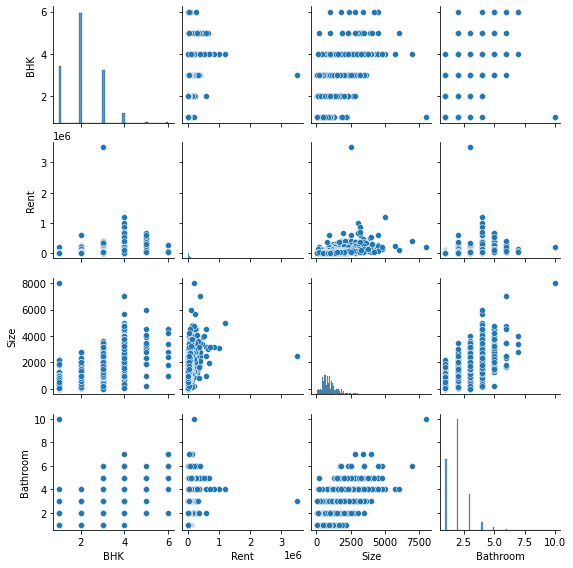
\includegraphics[width=0.7\textwidth]{Images/pairplot.png}
    \caption{Pairplot of data}
\end{figure}

A univariate and bivariate analysis was done to flush out outliers.~\cite{house-rent-prediction-model}\par\medskip

\noindent
\textbf{Rent (Our Target Variable)}
\begin{lstlisting}[language=python]
    fig = px.histogram(rent_data,x='Rent',color_discrete_sequence = px.colors.qualitative.Set3, title="Rent Prices Distribution Histogram")
    fig.show()
    fig = px.box(rent_data, x="Rent", title='Boxplot for Rent Prices')
    fig.show()
\end{lstlisting}

\clearpage
\begin{figure}[h]
    \centering
    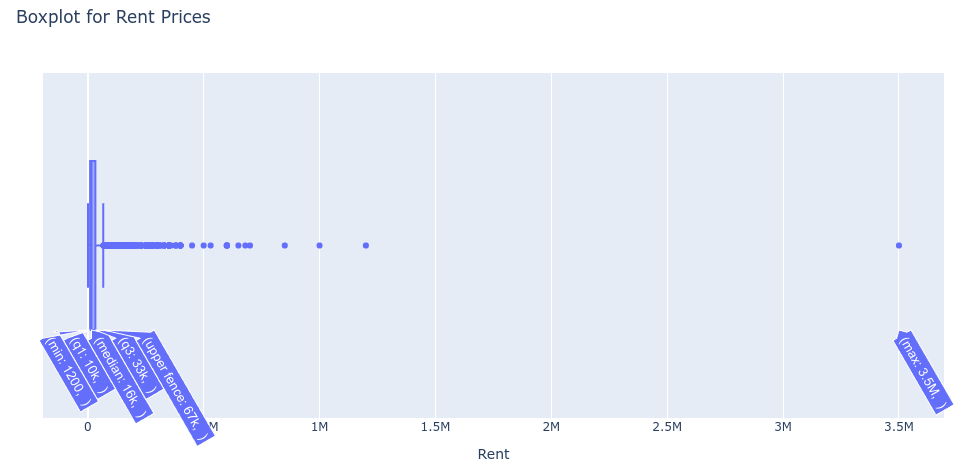
\includegraphics[width=0.7\textwidth]{Images/boxplotrent.png}
\end{figure}

\noindent\textbf{Observations:}
There is one outlier so far out of the inter-quantile range.
\medskip
\noindent\textbf{Actions:}
To remove outlier, as it may affect our assumptions about other variables and analysis

\begin{lstlisting}[language=python]
    print(np.where(rent_data['Rent']>2000000))
\end{lstlisting}

\noindent\textbf{Observations:}
Outlier's position is at 1837th position in a dataframe.
\medskip
\noindent\textbf{Deleting the outlier}
\begin{lstlisting}[language=python]
    rent_data.drop([1837], axis=0, inplace=True)

    fig = px.box(rent_data, x="Rent",title='Boxplot for Rent Prices')
    fig.show()
\end{lstlisting}

\noindent\textbf{BHK}
\begin{lstlisting}[language=python]
    rent_data['BHK'].value_counts()rent_data['BHK'].value_counts()
\end{lstlisting}


\begin{lstlisting}[language=python]
    sns.set_style('whitegrid')
    fig,axes = plt.subplots(figsize=(12,8))
    colors = ['#87ace8','#e3784d', '#6ecc64','#b644e3','#eb7c87', '#EAE509']
    
    ax = sns.countplot(x='BHK',data=rent_data, palette=['#e3784d','#87ace8', '#6ecc64','#b644e3','#eb7c87','#EAE509'])
    for container in ax.containers:
        ax.bar_label(container)
    plt.title('Frequency of different number of BHKs present in Houses available for Rent',fontsize=15)
    plt.show()
    
    fig = px.pie(rent_data, names='BHK', height=700, width= 700, color_discrete_sequence=px.colors.sequential.deep, title='Pie Chart for different number of BHKs present in Houses available for Rent')
    fig.update_traces(textfont_size=15)
    fig.show()
\end{lstlisting}

\begin{figure}[h]
    \centering
    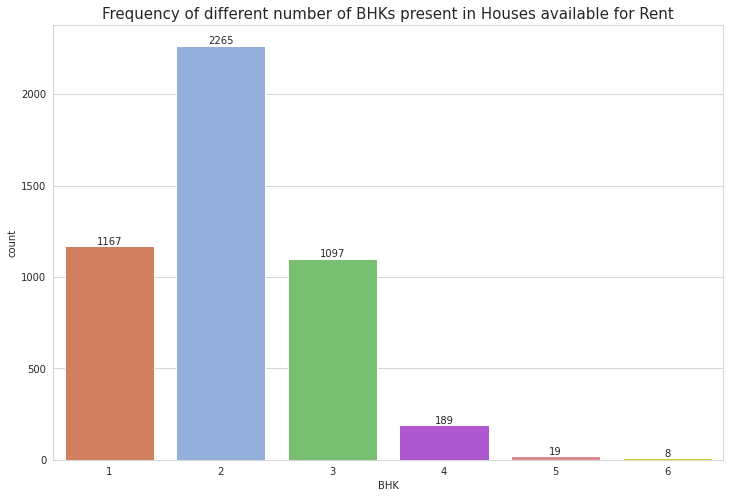
\includegraphics[width=0.7\textwidth]{Images/bhkfreq.png}
\end{figure}

\noindent\textbf{Observations:}
House with 2 Bathrooms are most common for the houses put up on rent. Houses with 7 and 10 bathroom quite seems inappropriate and not much of use.
\medskip

\noindent\textbf{City}
\begin{lstlisting}[language=python]
    rent_data['City'].value_counts()
\end{lstlisting}


\begin{lstlisting}[language=python]
    sns.set_style('whitegrid')
    fig,axes = plt.subplots(figsize=(12,8))
    colors = ['#87ace8','#e3784d', '#6ecc64','#b644e3','#eb7c87', '#EAE509']
    
    ax = sns.countplot(x='City',data=rent_data, palette=['#EAE509','#87ace8', '#6ecc64','#eb7c87','#e3784d','#b644e3'])
    for container in ax.containers:
        ax.bar_label(container)
    plt.title('City wise Houses available for Rent',fontsize=15)
    plt.show()
    
    fig = px.pie(rent_data, names='City', height=700, width= 700, color_discrete_sequence=px.colors.sequential.deep, title='Pie Chart for Houses available for Rent in different cities')
    fig.update_traces(textfont_size=15)
    fig.show()
\end{lstlisting}

\begin{figure}[h]
    \centering
    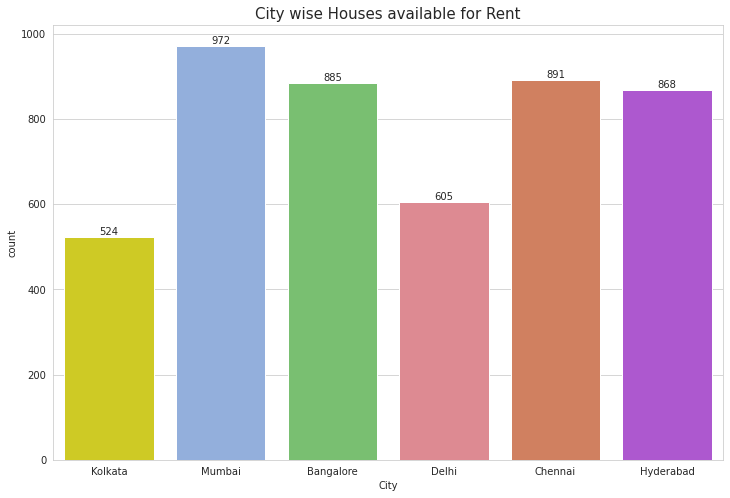
\includegraphics[width=0.7\textwidth]{Images/citygraph.png}
\end{figure}

\noindent\textbf{Observations:}
Mumbai, followed by Chennai and Hyderad has most number of rented houses, seems like there is very high demand considering the job corporates and other factors.
\medskip

\noindent\textbf{Liner Regression}\par
\noindent\medskip
A Linear Regression model was used to predict the prices in our application.\par
\medskip
The most extensively used modelling technique is linear regression, which assumes a linear connection between a dependent variable (Y) and an independent variable (X). It employs a regression line, also known as a best-fit line. The linear connection is defined as Y = c+m*X + e, where ‘c’ denotes the intercept, ‘m’ denotes the slope of the line, and ‘e’ is the error term.\par
\medskip
The linear regression model can be simple (with only one dependent and one independent variable) or complex (with numerous dependent and independent variables) (with one dependent variable and more than one independent variable).

\medskip
\noindent\textbf{Training the model}\par\medskip
\noindent\medskip
The model was trained using the following code:

\begin{lstlisting}[language=python]
    def predict_price(location,Size,bath,BHK):
    loc_index = np.where(X.columns == location)[0][0]
    
    x = np.zeros(len(X.columns))
    x[0]= BHK
    x[1]= Size
    x[2]= bath 
    if loc_index >=0:
        x[loc_index]=1
    
    return lr_clf.predict([x])[0]
\end{lstlisting}

using linear regression model we created a function to predict rental prices
\begin{lstlisting}[language=python]
    import pickle
    with open('rent_prices_model.pickle','wb') as f:
    pickle.dump(lr_clf,f)
\end{lstlisting}

\medskip
\noindent
After training our model we exported model as a pickel file so that we can load it in our flask server
we also exported json file containing all available locations in our model

\begin{lstlisting}[language=python]
    import json
    import pickle
    import numpy as np
    import sklearn
     
    __locations = None
    __data_columns = None
    __model = None
     
    def get_estimated_price(location,sqft,bath,bhk):
        try:
            loc_index = __data_columns.index(location.lower())
        except:
            loc_index =-1
        x= np.zeros(len(__data_columns))
        x[0]= bhk
        x[1]= sqft
        x[2]= bath
        if loc_index >=0:
            x[loc_index]=1
     
        return round(__model.predict([x])[0],2)
     
    def get_location_name():
        return __locations
     
    def load_saved_artifacts():
        print("loading saved artifacts... start")
        global __data_columns
        global __locations
     
        with open("./artifacts/columns.json",'r') as f:
           __data_columns= json.load(f)['data_columns']
           __locations = __data_columns[3:]
     
        global __model
        with open("./artifacts/rent_prices_model_1.pickle",'rb') as f:
            __model = pickle.load(f)
        print("loading saved artifacts...done")
     
    if __name__ == '__main__':
        load_saved_artifacts()
        print(get_location_name())
        print(get_estimated_price('Adambakkam',1200,2,3))
     
\end{lstlisting}
